% !TeX program = xelatex
\documentclass[UTF8,a4paper,11pt]{ctexart}
\usepackage[margin=1.8cm]{geometry}
\usepackage{amsmath,amssymb,mathtools}
\usepackage{enumitem,booktabs,longtable,xcolor,hyperref,tikz}
\usetikzlibrary{arrows.meta,calc,angles,quotes,positioning}
\hypersetup{hidelinks}
\setlist{leftmargin=2em,itemsep=0.25em}
\newcommand{\source}[1]{\par\smallskip\noindent\textcolor{gray}{\footnotesize 题源：#1}\par}
\newcommand{\lesson}[1]{\section{#1}}

\title{圆锥曲线专题教案：解析几何主线}
\author{教师复核稿}
\date{2026 年 8 月}

\begin{document}
\maketitle

\begin{quote}
本专题面向完成圆锥曲线基本概念学习后的复习与提升。课堂只使用普通高中解析几何中可书写、可评分的方法：定义、标准方程与几何性质、直线与曲线联立、判别式、韦达定理、点差法、向量与必要的平面几何。射影几何材料仅作为教师延伸阅读，不进入学生的必备方法链。
\end{quote}

\section*{专题结构与使用方式}
\begin{longtable}{p{0.13\textwidth}p{0.25\textwidth}p{0.31\textwidth}p{0.20\textwidth}}
\toprule
课时 & 核心任务 & 主要方法与典型障碍 & 当堂证据 \\
\midrule
1 & 定义、方程与性质复原 & 把焦点、准线、$a,b,c,e$ 的含义混用 & 能由条件选出曲线和首选工具 \\
2 & 定义的翻译与轨迹 & 忽略椭圆/双曲线定义的取值条件 & 能完整写出轨迹方程及限制 \\
3 & 直线与圆锥曲线 & 联立后漏掉判别式、弦长方向因子 & 能说明交点个数和弦长来源 \\
4 & 中点、定点与定值 & 只代入坐标而不利用两根结构 & 能用韦达或点差消去交点 \\
5 & 焦点弦、焦点三角形与最值 & 将焦半径、焦距、弦长混为一量 & 能先画出主三角形再列关系 \\
6 & 切线与综合表达 & 只报结论、不写存在性和取值范围 & 能完成一题规范书面表达 \\
\bottomrule
\end{longtable}

每课时按 45 分钟设计。若学校采用连堂课，可将第 3--4 课或第 5--6 课合并，并在中间安排 8--10 分钟限时书写。课堂练习使用同目录的《圆锥曲线专题练习：高考真题分类》；其中题干、答案与解析均应以所列本地题源复核。该练习已移除未经题设反算验证的自动示意图。

\section*{图形使用规范}
\begin{enumerate}
  \item 先由方程或几何条件确定图形，再标点和连线；不能先画图、后猜条件。
  \item 图上标出的点必须满足所属曲线或直线方程；标出的垂直、平行、相等关系必须能由题设或计算推出。
  \item 图形只辅助识别位置与结构，不能替代证明。涉及原卷题图时，以原卷为准。
\end{enumerate}

\begin{center}
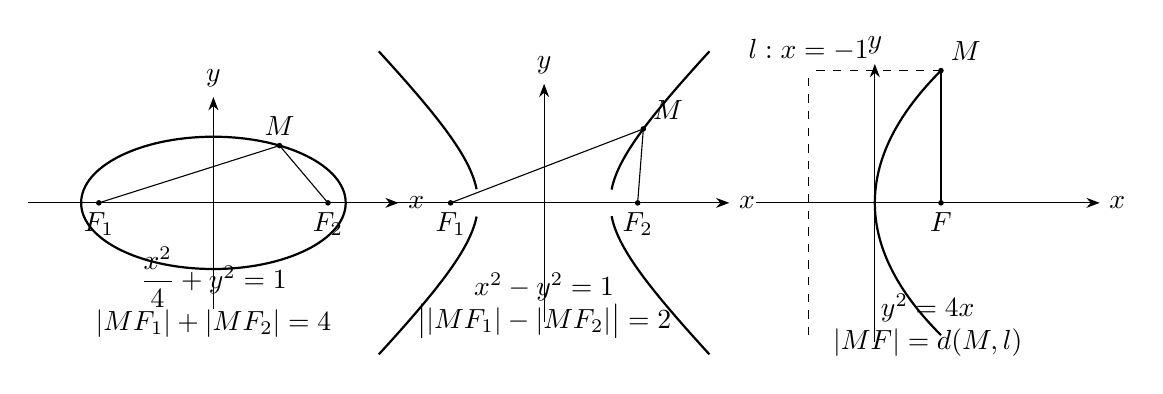
\begin{tikzpicture}[scale=0.84,>=Stealth]
  % Ellipse: x^2/4+y^2=1, foci (+-sqrt(3),0), M=(1,sqrt(3)/2).
  \begin{scope}[xshift=-5cm]
    \draw[->] (-2.8,0)--(2.8,0) node[right] {$x$};
    \draw[->] (0,-1.6)--(0,1.6) node[above] {$y$};
    \draw[thick] (0,0) ellipse (2 and 1);
    \fill (-1.732,0) circle (1.2pt) node[below] {$F_1$};
    \fill (1.732,0) circle (1.2pt) node[below] {$F_2$};
    \fill (1,0.866) circle (1.2pt) node[above] {$M$};
    \draw (1,0.866)--(-1.732,0) (1,0.866)--(1.732,0);
    \node[align=center] at (0,-1.35) {$\dfrac{x^2}{4}+y^2=1$\\$|MF_1|+|MF_2|=4$};
  \end{scope}
  % Hyperbola: x^2-y^2=1, foci (+-sqrt(2),0).
  \begin{scope}[xshift=0cm]
    \draw[->] (-2.8,0)--(2.8,0) node[right] {$x$};
    \draw[->] (0,-1.8)--(0,1.8) node[above] {$y$};
    \draw[thick,domain=-2.5:-1.02,samples=100,smooth] plot (\x,{sqrt(\x*\x-1)});
    \draw[thick,domain=-2.5:-1.02,samples=100,smooth] plot (\x,{-sqrt(\x*\x-1)});
    \draw[thick,domain=1.02:2.5,samples=100,smooth] plot (\x,{sqrt(\x*\x-1)});
    \draw[thick,domain=1.02:2.5,samples=100,smooth] plot (\x,{-sqrt(\x*\x-1)});
    \fill (-1.414,0) circle (1.2pt) node[below] {$F_1$};
    \fill (1.414,0) circle (1.2pt) node[below] {$F_2$};
    \fill (1.5,1.118) circle (1.2pt) node[above right] {$M$};
    \draw (1.5,1.118)--(-1.414,0) (1.5,1.118)--(1.414,0);
    \node[align=center] at (0,-1.55) {$x^2-y^2=1$\\$\bigl||MF_1|-|MF_2|\bigr|=2$};
  \end{scope}
  % Parabola: y^2=4x, focus (1,0), directrix x=-1.
  \begin{scope}[xshift=5cm]
    \draw[->] (-1.8,0)--(3.4,0) node[right] {$x$};
    \draw[->] (0,-2.1)--(0,2.1) node[above] {$y$};
    \draw[thick,domain=-2:2,samples=100,smooth,variable=\t] plot ({\t*\t/4},{\t});
    \draw[dashed] (-1,-2)--(-1,2) node[above] {$l:x=-1$};
    \fill (1,0) circle (1.2pt) node[below] {$F$};
    \fill (1,2) circle (1.2pt) node[above right] {$M$};
    \draw (1,2)--(1,0);
    \draw[dashed] (1,2)--(-1,2);
    \node[align=center] at (0.8,-1.85) {$y^2=4x$\\$|MF|=d(M,l)$};
  \end{scope}
\end{tikzpicture}
\end{center}
\noindent\small 图 1：三种定义图。标点均满足所画方程；图形用于定义复原，不代表任一原卷题图。\normalsize

\lesson{第 1 课：定义、标准方程与几何量复原}
\subsection*{目标}
学生能在椭圆、双曲线、抛物线之间完成“定义 -- 标准方程 -- 焦点/准线 -- 离心率”的双向翻译，并能说清 $a,b,c,p$ 分别由什么几何量确定。

\subsection*{教学流程}
\begin{enumerate}
  \item 5 分钟：不给公式，要求学生用一句话区别三种第一定义；追问椭圆和双曲线何时退化或无轨迹。
  \item 12 分钟：以图 1 复原 $c^2=a^2-b^2$、$c^2=a^2+b^2$、$y^2=2px$ 的焦点与准线。板书时固定写明 $a>b>0$、$p>0$ 等条件。
  \item 15 分钟：处理“已知点到焦点和准线的距离”类题。先让学生圈出距离对象，再决定是否调用抛物线定义；禁止一开始就设过多未知数。
  \item 8 分钟：限时完成两道选择题，交换答案并说明每一步依据。
  \item 5 分钟：出口题：写出 $y^2=8x$ 的焦点、准线，并解释为什么点到直线 $x=-3$ 的距离不能直接当作焦半径。
\end{enumerate}

\subsection*{课堂练习与评价}
\begin{itemize}
  \item 2023 北京卷第 6 题：考查第二定义与“距离对象不是准线”的辨析。
  \item 2022 全国乙卷（理）第 5 题：考查把 $|AF|=|BF|$ 转回准线距离。
\end{itemize}
成功标准：学生答案中必须写出准线方程或相应距离差，不能只凭图形报数。若错误集中在焦点坐标，下一课开始前用 3 分钟补做“由 $2p$ 定焦点”口答。

\lesson{第 2 课：定义翻译、轨迹与隐含曲线}
\subsection*{目标}
学生能识别距离和、距离差、点到直线距离和向量缩放条件；能写出轨迹方程、必要的取值限制及曲线名称。

\subsection*{教学流程}
\begin{enumerate}
  \item 8 分钟：比较“距离和为常数”“距离差绝对值为常数”“两距离相等”三类语言，要求学生先比较常数与焦距。
  \item 15 分钟：示范 2017 全国 II 卷（理）第 20 题第（1）问。只设 $M(x_0,y_0)$ 与 $P(x,y)$，从向量关系得到 $x=x_0,y=\sqrt2y_0$，再代回椭圆方程；强调得到方程后仍要说出轨迹是圆。
  \item 12 分钟：用 2016 全国 I 卷（理）第 20 题讨论椭圆定义。板书必须保留 $y\ne0$，并说明这一限制来自原构造中直线不与 $x$ 轴重合。
  \item 10 分钟：两人一组互改“轨迹结论句”，检查是否同时包含方程、曲线名称和限制。
\end{enumerate}

\subsection*{易错点}
把 $|MF_1|+|MF_2|=2a$ 一出现就写椭圆，而不检查 $2a>|F_1F_2|$；消元时平方造成增根却不回代；只写方程而不交代去掉的端点或直线。评价时按“关系翻译、代数变形、结论完整”三个点分别记录，不把三类错误混作粗心。

\lesson{第 3 课：直线与圆锥曲线的位置关系和弦长}
\subsection*{目标}
学生能用联立和判别式判断交点个数，能说明弦长公式中的方向因子来自两点间距离，而不是把横坐标差直接当弦长。

\begin{center}
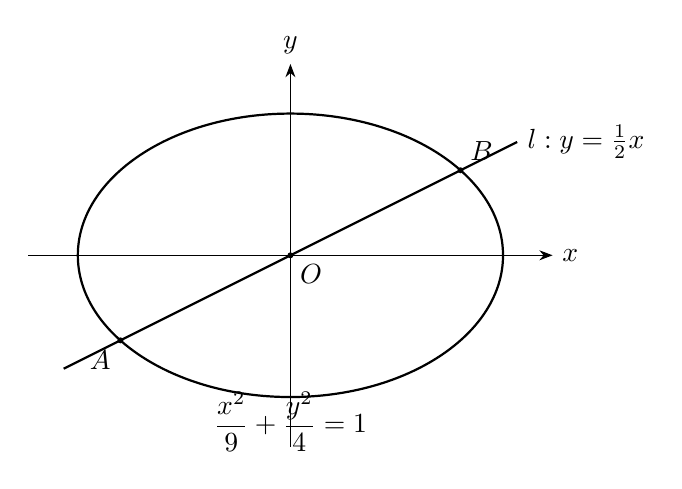
\begin{tikzpicture}[scale=0.9,>=Stealth]
  \draw[->] (-3.7,0)--(3.7,0) node[right] {$x$};
  \draw[->] (0,-2.7)--(0,2.7) node[above] {$y$};
  \draw[thick] (0,0) ellipse (3 and 2);
  \draw[thick] (-3.2,-1.6)--(3.2,1.6) node[right] {$l:y=\frac12x$};
  \fill (-2.4,-1.2) circle (1.2pt) node[below left] {$A$};
  \fill (2.4,1.2) circle (1.2pt) node[above right] {$B$};
  \fill (0,0) circle (1.2pt) node[below right] {$O$};
  \draw[dashed] (-2.4,-1.2)--(2.4,1.2);
  \node at (0,-2.35) {$\dfrac{x^2}{9}+\dfrac{y^2}{4}=1$};
\end{tikzpicture}
\end{center}
\noindent\small 图 2：直线 $y=\frac12x$ 与椭圆 $\frac{x^2}{9}+\frac{y^2}{4}=1$ 的交点为 $(-\frac{12}{5},-\frac65)$、$(\frac{12}{5},\frac65)$，均已代入核对。\normalsize

\subsection*{教学流程}
\begin{enumerate}
  \item 10 分钟：以图 2 说明“有两个交点”既可以由图形预判，也必须由 $\Delta>0$ 代数确认。
  \item 15 分钟：板书通法：设直线、联立、整理为一元二次、判别式、韦达、回到几何量。每一步注明变量含义。
  \item 12 分钟：处理弦中点题时，先区分“中点坐标已知”和“中点在定直线上”两种信息，再选择韦达或点差。
  \item 8 分钟：限时完成 2023 全国乙卷（理）第 11 题和 2016 全国 III 卷（文）第 20 题的第一问。
\end{enumerate}

\lesson{第 4 课：点差法、定点与定值}
\subsection*{目标}
学生能解释点差法的来源：两交点分别代入同一曲线方程后相减，从而把二次项化为含中点坐标的线性关系；能在定点题中区分“代入验证”和“消元证明”。

\subsection*{教学流程}
\begin{enumerate}
  \item 8 分钟：先用两点 $P(x_1,y_1),Q(x_2,y_2)$ 代入椭圆方程并相减，要求学生自己完成因式分解。
  \item 17 分钟：用 2017 全国 I 卷（理）第 20 题练习“设直线 -- 联立 -- 韦达 -- 消去参数”。每次约分前提示检查分母是否为零。
  \item 12 分钟：用 2020 全国 I 卷（理）第 20 题比较两条路线：坐标消元与结构性观察。答案以能评分的坐标过程为准。
  \item 8 分钟：书写诊断。学生只交最后 8 行推导，教师按是否设清变量、是否保留参数范围、是否验证定点三项批注。
\end{enumerate}

\lesson{第 5 课：焦点三角形、焦点弦与最值}
\subsection*{目标}
学生能先确定真正承载条件的三角形，再选择余弦定理、面积公式、抛物线定义或参数法；能检查焦点弦的端点是否属于同一支及最值等号能否取得。

\begin{center}
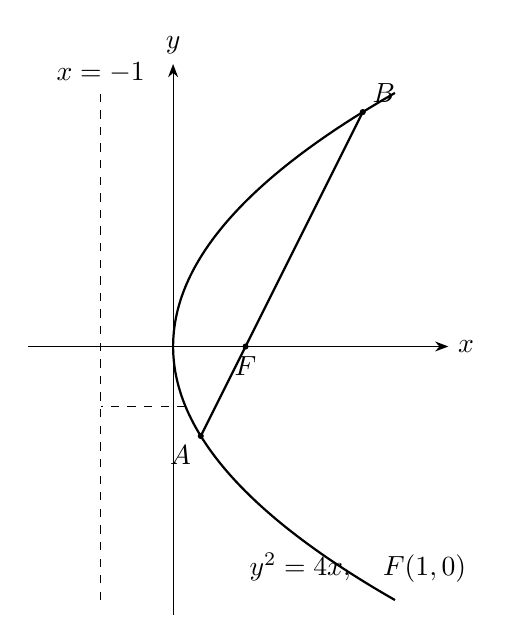
\begin{tikzpicture}[scale=0.92,>=Stealth]
  \draw[->] (-2,0)--(3.8,0) node[right] {$x$};
  \draw[->] (0,-3.7)--(0,3.9) node[above] {$y$};
  \draw[thick,domain=-3.5:3.5,samples=120,smooth,variable=\t] plot ({\t*\t/4},{\t});
  \draw[dashed] (-1,-3.5)--(-1,3.5) node[above] {$x=-1$};
  \fill (1,0) circle (1.2pt) node[below] {$F$};
  \coordinate (A) at (0.382,-1.236);
  \coordinate (B) at (2.618,3.236);
  \draw[thick] (A)--(B);
  \fill (A) circle (1.2pt) node[below left] {$A$};
  \fill (B) circle (1.2pt) node[above right] {$B$};
  \draw[dashed] (0.172,-0.828)--(-1,-0.828);
  \node at (2.55,-3.05) {$y^2=4x,\quad F(1,0)$};
\end{tikzpicture}
\end{center}
\noindent\small 图 3：焦点弦 $AB$ 取直线 $y=2(x-1)$ 与 $y^2=4x$ 的交点，图中 $F(1,0)$ 在弦上；端点坐标为近似值，仅用于结构识别。\normalsize

\subsection*{教学流程}
\begin{enumerate}
  \item 10 分钟：让学生在图 3 上标出焦半径、焦距、弦长，说明三者不是同一个量。
  \item 15 分钟：以 2020 全国 II 卷（理）第 19 题说明焦点、椭圆和抛物线共用坐标系时，先由第（1）问确定离心率，再进入第（2）问。
  \item 12 分钟：用 2019 全国 I 卷（理）第 10 题练习由椭圆定义还原三角形边长，再使用余弦定理。
  \item 8 分钟：对最值题逐项检查：可行域、等号条件、所得点是否满足原限制。
\end{enumerate}

\lesson{第 6 课：切线、综合题与规范表达}
\subsection*{目标}
学生能写出椭圆切线的正确形式，明确切点条件；在综合题中保持“设元 -- 联立 -- 关系 -- 结论”的可评分链条，并能够复核图形是否支持结论。

\subsection*{教学流程}
\begin{enumerate}
  \item 8 分钟：回顾椭圆 $\frac{x^2}{a^2}+\frac{y^2}{b^2}=1$ 在 $(x_0,y_0)$ 处的切线公式，先强调 $(x_0,y_0)$ 必须在椭圆上。
  \item 15 分钟：完成 2021 天津卷第 18 题。重点检查“与 $y$ 轴正半轴相交”给出的符号限制，避免只解出直线而漏筛选。
  \item 15 分钟：完成 2023 新高考 II 卷第 21 题的一个书写片段。要求先写参数范围，再用韦达表达对称量，最后验证定直线。
  \item 7 分钟：专题小结。学生写下本专题最容易漏掉的一个限制条件，并给出一题中对应的具体位置。
\end{enumerate}

\section*{课后分层作业与复核}
\begin{itemize}
  \item 基础：2023 北京卷第 6 题、2022 全国乙卷（理）第 5 题、2023 全国乙卷（理）第 11 题。目标是定义和直线联立的规范表达。
  \item 巩固：2017 全国 II 卷（理）第 20 题、2020 全国 II 卷（理）第 19 题。目标是轨迹转化与焦点结构。
  \item 提升：2021 天津卷第 18 题、2023 新高考 II 卷第 21 题。目标是参数范围、切线与定点证明。
\end{itemize}

批改时只记录可观察证据：定义对象是否写对、方程是否带条件、消元是否保留等价性、最终结论是否回应问题。不要把未核实的学生表现写成统计结论。新题或改题进入正式题库前，应再次对照原卷题干、答案、图形和评分规则。

\source{本地题库：\texttt{高考真题/tex版(exam-zh模板2016-2025)/年份/卷别/questions.json}}
\end{document}
